%%%%%%%%%%%%%%%%%%%%%%%%%%%%%%%%%%%%%%%%%
% Journal Article
% LaTeX Template
% Version 1.3 (9/9/13)
%
% This template has been downloaded from:
% http://www.LaTeXTemplates.com
%
% Original author:
% Frits Wenneker (http://www.howtotex.com)
%
% License:
% CC BY-NC-SA 3.0 (http://creativecommons.org/licenses/by-nc-sa/3.0/)
%
%%%%%%%%%%%%%%%%%%%%%%%%%%%%%%%%%%%%%%%%%

%----------------------------------------------------------------------------------------
%	PACKAGES AND OTHER DOCUMENT CONFIGURATIONS
%----------------------------------------------------------------------------------------

\documentclass[twoside]{article}

\usepackage{lipsum} % Package to generate dummy text throughout this template

\usepackage{graphicx}
\graphicspath{ {Screenshots/} }
\usepackage[export]{adjustbox}

\usepackage[sc]{mathpazo} % Use the Palatino font
\usepackage[T1]{fontenc} % Use 8-bit encoding that has 256 glyphs
\linespread{1.05} % Line spacing - Palatino needs more space between lines
\usepackage{microtype} % Slightly tweak font spacing for aesthetics

\usepackage[hmarginratio=1:1,top=32mm,columnsep=20pt]{geometry} % Document margins
\usepackage{multicol} % Used for the two-column layout of the document
\usepackage[hang, small,labelfont=bf,up,textfont=it,up]{caption} % Custom captions under/above floats in tables or figures
\usepackage{booktabs} % Horizontal rules in tables
\usepackage{float} % Required for tables and figures in the multi-column environment - they need to be placed in specific locations with the [H] (e.g. \begin{table}[H])
\usepackage{hyperref} % For hyperlinks in the PDF

\usepackage{lettrine} % The lettrine is the first enlarged letter at the beginning of the text
\usepackage{paralist} % Used for the compactitem environment which makes bullet points with less space between them

\usepackage{abstract} % Allows abstract customization
\renewcommand{\abstractnamefont}{\normalfont\bfseries} % Set the "Abstract" text to bold
\renewcommand{\abstracttextfont}{\normalfont\small\itshape} % Set the abstract itself to small italic text

\usepackage{titlesec} % Allows customization of titles
\renewcommand\thesection{\Roman{section}} % Roman numerals for the sections
\renewcommand\thesubsection{\Roman{subsection}} % Roman numerals for subsections
\titleformat{\section}[block]{\large\scshape\centering}{\thesection.}{1em}{} % Change the look of the section titles
\titleformat{\subsection}[block]{\large}{\thesubsection.}{1em}{} % Change the look of the section titles

\usepackage{fancyhdr} % Headers and footers
\pagestyle{fancy} % All pages have headers and footers
\fancyhead{} % Blank out the default header
\fancyfoot{} % Blank out the default footer
\fancyhead[C]{Mental Models Analysis: Ubiquitous Computing $\bullet$ October 2014} % Custom header text
\fancyfoot[RO,LE]{\thepage} % Custom footer text

%----------------------------------------------------------------------------------------
%	TITLE SECTION
%----------------------------------------------------------------------------------------

\title{\vspace{-15mm}\fontsize{24pt}{10pt}\selectfont\textbf{Ubiquitous Learning}} % Article title

\author{
\large
\textsc{Jackson Souza}\\[2mm] % Your name
\normalsize Loyola Marymount University \\ % Your institution
\normalsize CMSI 370: Dr. Dionisio \\ % Your institution
\vspace{-5mm}
}
\date{}

%----------------------------------------------------------------------------------------

\begin{document}

\maketitle % Insert title

\thispagestyle{fancy} % All pages have headers and footers

%----------------------------------------------------------------------------------------
%	ABSTRACT
%----------------------------------------------------------------------------------------

\begin{abstract}

\noindent  The recent emergence of ubiquitous computing has brought about a proposed revision of many fields, including education. This paper will examine ubiquitous learning as a subset of ubicomp and explain the similarities between the fields. U-learning amplifies specific, sought after traits in instruction that will be utilized to show the progress of the field. By examining how u-learning applications accommodate multiple user profiles and balance automation and control, we can asses their aptitude as intelligent spaces versus other applications of ubiquitous computing in the classroom. In examining these specific traits, we can validate the actual progress of abstract ideas in u-learning.

\end{abstract}

%----------------------------------------------------------------------------------------
%	ARTICLE CONTENTS
%----------------------------------------------------------------------------------------

\begin{multicols}{2} % Two-column layout throughout the main article text

\section{Introduction}

\lettrine[nindent=0em,lines=3]{T}he \emph{internet of things} (ITT) is a powerful and very real 21st century notion. The ubiquity of the technology that surrounds us is apparent in many fields, one of which hinges on usability to achieve its aims. The educative process is utterly dependent on \emph{transferring the system image} from instructor to student, which makes the field an excellent vantage point from which to examine ubiquitous computing. Much research has been dedicated to the relationship between ubicomp and education, as \emph{ubiquitous learning} (u-learning) is seen as the next natural step from e-learning and the traditional K-12 system. The methods used to communicate a system image via ubicomp are readily apparent in examining u-learning as a subset of ubicomp. Within the greater context of interaction design, ubicomp (and therefore, u-learning) communicates predictively by anticipating user actions, familiarity with the system and context, and receptivity.

%------------------------------------------------

\section{Background}

% JD: These repeated \setlength\parindent directives are not in the spirit of LaTeX.
%     If this is really how you want it, you should create a new document class or
%     preset the right variables.  Otherwise, leave well enough alone.
\setlength\parindent{24pt}The coinage \emph{ubiquitous learning} comes from a 2005 paper by Sakamura and Koshizuka, in which they define the term as \emph{a novel learning style [where] we [can] learn anything at anytime and anywhere utilizing ubiquitous computing technology and infrastructure.}\footnote{Sakamura, 1} To explain this idea, they imagine a plate, where when filled with food, could provide the user with information about where the food was grown, caloric content, ect. Champions of this learning style say that we now possess the technology the overhaul the traditional ways that information is presented, integrating them with the world around us. A departure from tradition depends on the creation of unique ways to present information, otherwise risking the same low retention rates. Sakamura and Koshizuka present mainly RFID or U-Code transmission of data from specific sites to a user's phone or tablet. 

\setlength\parindent{24pt}The aims and technologies harnessed by u-learning have not changed much, as phones and tablets have become king. Due to this large increase in the adoption of smart phones and tablets since 2005, the amount of specific \emph{on-site technologies} like QR-codes and RFID tags, repurposed to force information on a user (often via advertisement), have shot up astronomically. This corruption of simple site-based technologies and ubiquity of touchscreen devices has forced proponents of u-learning to create unique methods of information communication. Since Sakamura and Koshizuka, intermediary hardware and software between the learning site and the user`s chosen device has become the focus of ubicomp.

\setlength\parindent{24pt}Although similar, Wloka and Winiwarter\footnote{Wloka, 1} draw a distinction between u-learning and mobile learning.
\begin{flushleft}
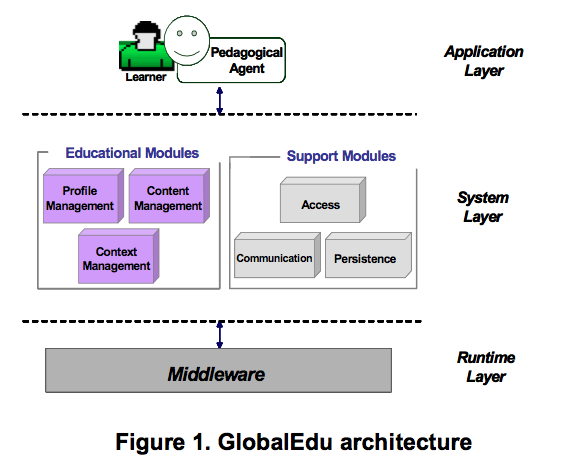
\includegraphics[scale=0.35,left]{1}
% JD: You should crop out the caption from the image and place the caption
%     here in the text.  Plus, the proper environment is figure, not flashlight.
\end{flushleft}
Not to be delineated by the chosen display device, u-learning is characteristic of a system that is highly embedded and highly mobile. Mobile learning is just mobile, where the information and system are contained within the device. The hallmark of u-learning is its ubiquity, echoing Sakamura: where information is available throughout an environment and can be accessed by the system at any time. This is why u-learning is suitable for a classroom or the home, places where the activities that happen within them are unique to the specific environment. To clarify this point, one may eat at the mall, but malls are made for shopping. Just as well, one may dance in the food court, but you come to the food court to eat, so providing a system with a specific environmental focus is common in ubicomp.

\setlength\parindent{24pt}Hua\footnote{Hua, 1} examines the types of ubiquitous computing used in u-learning and how the two intimately relate. He lists, \emph{At present the main application areas of ubiquitous computing include smart terminal devices (such as Mobile Web 2.0 applications on iPhones), intelligent space (such as smart classroom), and RFID tags for business identification and so on.} Hua emphasizes the importance of ubicomp as \emph{intelligent space}, seeking an alternative to the other methods listed, which, as discussed, have been all but devalued by advertisement and entertainment. He names this method \emph{ULO} or Ubiquitous Learning Object (or Environment), which is characterized by a wealth of resources, a friendly interface and most importantly, multidimensional environment and {perceived collaborative learning}. What Hua means by multidimensional is an environment characteristic of \emph{multiple modalities of learning. The master ratio of learners is different according to different ways of knowledge. If the learner involve in explanation directly, he (or she) can master more than seeing or hearing.} In other words, the ULO must be sensitive to the users preferred modes of interaction.

\setlength\parindent{24pt}Barbosa, Barbosa, Hahn and Geyer are able to abstract u-learning interaction into the following diagram for their GlobalEDU system, similar to Hua. The application layer is synonymous with the user`s chosen application and device. The runtime layer executes the application. The system layer is divided into two areas, with the educational modules managing the content and \emph{adapting the resources [the learner is] manipulating}\footnote{Barbosa, 3} while the support modules \emph{adapt the interfaces to devices, user`s access and persistence.} Adaptation is clearly the focus in GlobalEDU, predicting the user`s level of engagement with the system and the material.


%------------------------------------------------

\section{Methods}

\setlength\parindent{24pt}This predictive application of ubicomp characterizes much of u-learning, as the service that most u-learning software provides is adaptation of the information to the user, similar to what an instructor does. This process of actively shaping the learning experience can be best described by Norman`s \emph{Stages of Action} theory.\footnote{Wikipedia} 
\begin{flushleft}
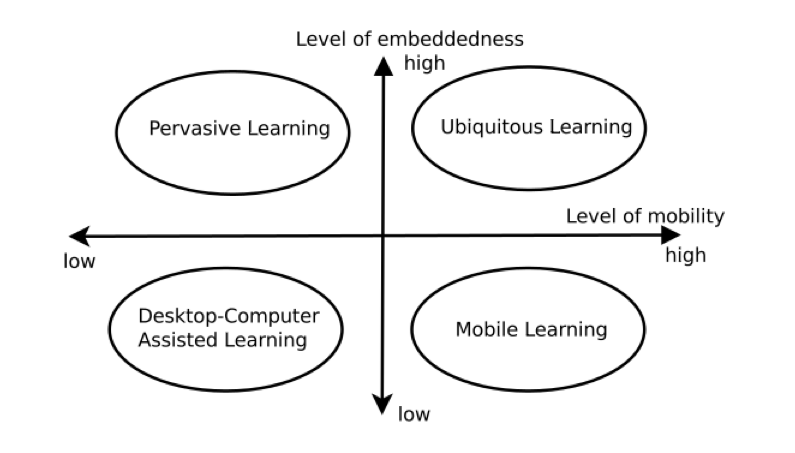
\includegraphics[scale=0.25,left]{2} 
\end{flushleft} 
Norman?s theory can be used to evaluate the adaptive aptitude of u-learning systems by examining the user profile, the user?s familiarity with context, content and the system, and accommodation of the user?s receptivity.
% JD: You may have copy-pasted the text from a word processor that uses "smart quotes."
%     As a result, apostrophes all appear as question marks here.  I'm a little surprised
%     that you just let this go---a quick scan of your PDF would have revealed the tweaked
%     encoding, and this would then be an easy search-replace fix.

\setlength\parindent{24pt}In examining the system put forth by Barbosa, Barbosa, Hahn and Geyer, GlobalEDU appears to explicitly address all steps of Norman`s theory. The educational modules support Norman`s stages of evaluation, while the support modules facilitate execution. To perceive the user profile (in this case, the user?s specific learning style), GlobalEDU uses the access and persistence submodules. Adapting the interface to a user?s rate of progress is also a responsibility of the persistence submodule. As for assessing the user`s context in the material and GlobalEDU system, the educational and support modules communicate through the context management submodule which, \emph{has the capability to know how to locate the learner in his/her current environment, to identify a learner in the corresponding context and to provide information adapted to the device the learner is using.}\footnote{Barbosa, 4}
 \begin{flushleft}
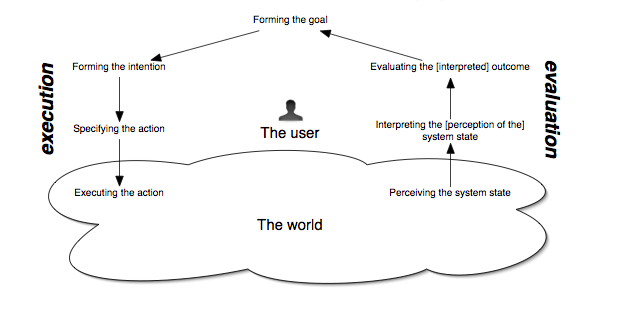
\includegraphics[scale=0.35,left]{3} 
\end{flushleft}

\setlength\parindent{24pt}The level of abstraction in the GlobalEDU system is very high and only really makes sense when you put it all in context. The authors describe a small u-learning situation where a \emph{Programming Languages} class forms groups for a debate. At the very least, the system was able to perform the clerical duties of a professor: taking attendance, distributing information among groups, adapting the context per language and for tardy students. In another situation they described, the system, based on historical and previous user profile data, was able to suggest learning resources tailored to the user on completion of an assignment. Both of these situations capitalize on Hua`s definitions for u-learning: having multiple modalities of learning and collaboration. Also, the system is driven by the user, but accurately scaled to a level of automation appropriate for the user, mimicking an instructor.

\setlength\parindent{24pt}Li, Chen, Gao and Huang have a slightly more complex system, named SULOM. This system seeks to \emph{systematize} the ULO concept as put forth by Hua. The structure of their ULO model is decidedly less about the actual process than GlobalEDU and much more about the semantics and ontology of ULOs.
\begin{flushright}

\includegraphics[scale=0.55,right]{4} 
\end{flushright} 
To explain more clearly, the authors give an example of ULOs incorporated into a course. 
\begin{flushright}
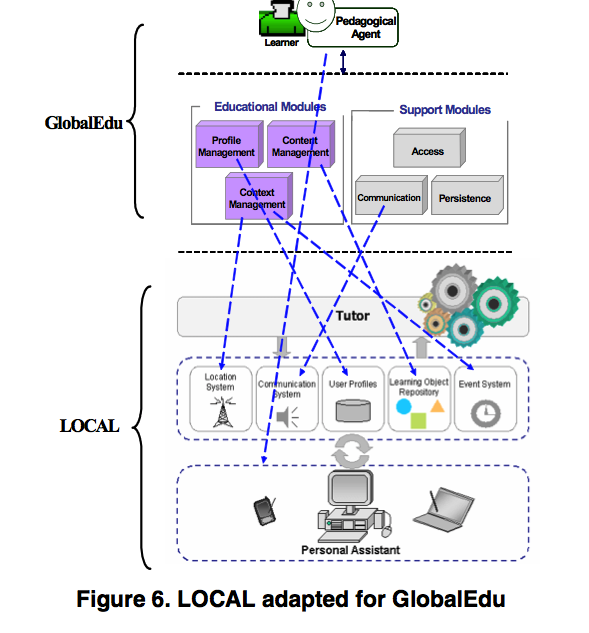
\includegraphics[scale=0.35,right]{5} 
\end{flushright}
Each point of knowledge represents a ULO, which is explained by the first figure. As opposed to GlobalEDU which proposes a specific system, SULOM tries a more philosophical approach at articulating what the metadata of specific knowledge might contain and how these points interconnect. I imagine that SULOMs might be used within GlobalEDU to move the system towards a more holistic, relational knowledge about its user base. U-Learning hinges on items 5 and 6 of Norman?s seven stages and SULOM is able to accurately represent how this is done.

\setlength\parindent{24pt}Finally, Chen, Hung and Wang have developed a system using robots to facilitate learning. Combining both higher level concepts as espoused in GlobalEDU and lower-level epistemological concerns as addressed in SULOM, the authors are able to actually create a functioning \emph{intelligent space}. Harnessing the power of LEGO Mindstorms robots, Chen et al. created the U-One system affording young users, \emph{good learning motivations and more concentration on learning activities}\footnote{Chen, 2}. It was unclear how the researchers used the actual robots in their experiment, but besides this, the experiment was enough to show the power of u-learning. The researchers were able to effectively convey the concept of multiplication to 15 second-graders using Chinese checkers and RFID tags combined with custom software. A simple caveat that allowed the system to scale to the user profile was that students were able to assemble the checkers using addition (3 + 3 + 3) or multiplication (3 x 3) to reach the answer. In this way, adaptability was inherent in this very simple experiment, because no matter the level of arithmetic that the user was familiar with, they could grasp the concept through the avenue most conducive to their learning. 
% JD: The problem here so far is I'm not seeing actual *user interfaces*, against which
%     we can then have a discussion of mental model transfer and usability.  I get that
%     you are addressing the transference of mental models at a different level---that
%     of pedagogy---but that discussion remains conceptual and speculative in the absence
%     of empirical data or actual systems (in the paper).  I know that the works cited
%     did/built some concrete things, but that is not what this paper conveys.  Instead,
%     the focus is more on methodology and process, making the ideas harder to pin down.

%------------------------------------------------

\section{Discussion}

\setlength\parindent{24pt}	It is readily apparent that mental models being communicated and adapted in real time are the hallmarks of ubiquitous learning. Special attention is being paid to Norman`s steps 5 and 6:  \emph{perceiving and interpreting the state of the world.} It is also clear through a careful look at GlobalEDU, SULOM and U-One, that u-learning can be addressed at many different levels of abstraction and scope, although, some levels were more appropriate than the others at communicating ubicomp concepts. I would be quick to rule out SULOM as too abstract, leaning more towards the realm of metacognition in describing the learning ontology. SULOM did not present much of a system to analyze through previous research, although it did establish u-learning as highly relational. GlobalEDU and U-One were able to provide me a wealth of information, where U-One was able to put most of the GlobalEDU concepts into concrete applications.
% JD: OK, at least you thought so too :)  But that still begs the question of "where's
%     the interaction design" in this paper.

\setlength\parindent{24pt}	U-One did come off as a little too simplistic, much like the RFID tag and QR code laden experiments that had been discussed previously. I believe that this only in part due to the existing technology we have, as the ubiquity of tablets and smart phones have pigeon holed researchers into using such devices. Experiments like U-One chose to use their device as just a resource to display information and delegated the actual activity to the checkers pieces. Still, these harnessed RFID tags, where they could have used cameras, knobs, switches, etc. to expand the originality of the research. 
% JD: See, illustrations and discussions centering around the actual *apparatus* may
%     have been the better choice.  Instead, the perspective of overviews and diagrams
%     is taken, making the discussion less grounded.

\setlength\parindent{24pt}	Translating the GlobalEDU or SULOM systems into physical reality was shown as nearly impossible, due in large part to an attachment to the traditional setting of a classroom. As shown by U-One, it is extremely difficult to create a truly intelligent space instead of just a single, localized instance of learning.  These notions of relational learning and intelligent space are what should dominate u-learning experiments, but disappointingly, do not. In the abstract systems discussed, we clearly have an idea of what should be done, however our attachment to the traditional classroom limits the space and objects researchers work with.
% JD: Well I guess in the end I think you are seeing what I am also seeing---that the work
%     presented here is extremely preliminary and has not yet converged upon standard devices
%     or systems for which we can reason about mental model transfer and usability.  This
%     will be tricky to grade...on the one hand you chose to tackle a novel and interesting
%     variant of the subject, but on the other the findings have not lent themselves well to
%     interaction design or usability analysis.

%------------------------------------------------

\section{Conclusions}

\setlength\parindent{24pt}	Ubicomp is entrenched in education and there to stay. More and more, the ideas about the traditional classroom are giving way to u-learning`s intelligent space, opening up new possibilities for adaptation to students. Modifying these educational interactions with students in real time is the current height of u-learning put forth by systems like GlobalEDU, SULOM and U-One. Perceived collaboration, and tight synchronization with the user`s learning profile are the hallmarks of u-learning, and indicative of its deep relationship with ubicomp. Bringing the recent u-learning research into physical actuality is difficult, but intelligent space, sensitive to learners is slowly, but surely being developed as new technologies emerge.


%----------------------------------------------------------------------------------------
%	REFERENCE LIST
%----------------------------------------------------------------------------------------
% JD: Bummer, not BibTeX.  This is less reusable and semantic.
\begin{thebibliography}{99} % Bibliography - this is intentionally simple in this template

\bibitem AAll images belong to their respective articles.

\bibitem SSakamura, Ken. and Noboru Koshizuka. (2005).
\newblock Ubiquitous Computing Technologies for Ubiquitous Learning.
\newblock {\em 2005 IEEE International Workshop on Wireless and Mobile Technologies in Education}.

\bibitem WWloka, Bartholomäus, and Werner Winiwarter. (2010).
\newblock Enhancing Language Learning and Translation with Ubiquitous Applications.
\newblock {\em Mobile Applications: MoMM2010 Proceedings }.

\bibitem HHua, Zhang. (2010).
\newblock Study of Ubiquitous Learning Environment Based on Ubiquitous Computing.
\newblock {\em Tianjin University of Science and Technology: The Study of Multi-Agent's Application In Distributed Teaching System}.

\bibitem BBarbosa, Jorge, Rodrigo Hahn, Debora Barbosa, and Claudio Geyer. (2008).
\newblock Learning in Small and Large Ubiquitous Computing Environments.
\newblock {\em IEEE/IFIP International Conference on Embedded and Ubiquitous Computing}.

% JD: This is an online-only resource and should thus include a URL as well
%     as a date of last access.
\bibitem WWikipedia contributors. (2014).
\newblock Seven stages of action.
\newblock {\em Wikipedia, The Free Encyclopedia}.

\bibitem CChen, Nian-Shing, I-Chun Hung, and Chun-Wang Wei. (2010).
\newblock Developing Ubiquitous Learning System with Robots for Children's Learning.
\newblock {\em 2010 IEEE International Conference on Digital Game and Intelligent Toy Enhanced Learning }.
 
\end{thebibliography}

%----------------------------------------------------------------------------------------

\end{multicols}

\end{document}
